
\chapter{標準化残存率モデルの構築と統計解析}

%--------------------------------------------------
\section{本章の目的}

第5章では、
掌面積による標準化を施した残存率を用いて、
洗浄条件の違いがMS2ファージの除去効率に及ぼす影響を評価した。
その結果、
洗浄回数の増加に伴い残存率が低下する傾向が確認された一方で、
被験者ごとに残存率のばらつきが存在するように見受けられた。

そこで本章では、
第5章で得られた標準化残存率データを対象として、
統計解析を行い、
個人差および洗浄回数が残存率に与える影響を定量的に評価することを目的とする。
具体的には、
二元配置分散分析およびTukeyの多重比較検定を用いて、
被験者間の差および洗浄回数条件間の差を検証する。

さらに、
統計解析によって得られた結果をもとに、
残存率を確率分布として整理し、
後続章における感染リスク評価（QMRA）に用いる
入力分布を構築する。
%--------------------------------------------------
\section{使用データと解析条件}

本章で使用したデータは、
第5章において算出した掌面積で標準化された残存率である。
対象となるデータは以下の条件で構成される。

\begin{itemize}
  \item 被験者：5名
  \item 手の別：右手、左手
  \item 洗浄回数：1～5回
  \item 繰り返し測定：各条件4回
\end{itemize}

1つの洗浄回数条件につき、
5名 $\times$ 2手 $\times$ 4回 = 40データが存在する。
本解析では、
これらの残存率データを用いて、
洗浄回数および個人差の影響を検討した。
%--------------------------------------------------
\section{二元配置分散分析による検証}

標準化残存率に対する個人差および洗浄条件の影響を評価するため、
二元配置分散分析を実施した。
解析では、
被験者および手の別を要因として設定し、
洗浄回数ごとに残存率の違いを検証した。

\begin{table}[htbp]
  \centering
  \caption{洗浄回数ごとの二元配置分散分析結果}
  \label{tab:anova_wash_each}
  \small
  \begin{tabular}{c l c c c}
    \hline
    洗浄回数 & 要因 & 自由度 & $F$値 & $p$値 \\
    \hline
    1 & 被験者        & 4 & 1.79 & 0.160 \\
      & 手            & 1 & 3.61 & 0.068 \\
      & 被験者$\times$手 & 4 & 0.86 & 0.499 \\
    \hline
    2 & 被験者        & 4 & 1.39 & 0.263 \\
      & 手            & 1 & 2.16 & 0.153 \\
      & 被験者$\times$手 & 4 & 1.27 & 0.306 \\
    \hline
    3 & 被験者        & 4 & 1.38 & 0.266 \\
      & 手            & 1 & 1.92 & 0.178 \\
      & 被験者$\times$手 & 4 & 1.36 & 0.275 \\
    \hline
    4 & 被験者        & 4 & 1.42 & 0.254 \\
      & 手            & 1 & 1.78 & 0.193 \\
      & 被験者$\times$手 & 4 & 1.43 & 0.250 \\
    \hline
    5 & 被験者        & 4 & 1.40 & 0.261 \\
      & 手            & 1 & 1.89 & 0.180 \\
      & 被験者$\times$手 & 4 & 1.51 & 0.227 \\
    \hline
  \end{tabular}
\end{table}

表\ref{tab:anova_wash_each}に、洗浄回数ごとに実施した二元配置分散分析の結果を示す。
いずれの洗浄回数においても、被験者の主効果、手（左右）の主効果、
ならびに被験者と手の交互作用はいずれも統計的に有意ではなかった（すべて $p > 0.05$）。
この結果から、洗浄回数を固定した条件下では、
残存率に対する個人差および左右差の影響は統計的に有意ではなく、
残存率の変動は主として洗浄回数そのものに依存していると考えられる。

洗浄回数による多重比較を行う前に
洗浄回数を要因とした残存率データについて、
分散分析の前提条件を確認するため、正規性および等分散性の検定を行った。
Shapiro–Wilk検定の結果、残存率の分布は正規分布に従わないことが示された
（W = 0.946, p < 0.001）。
これは残存率が0から1の範囲に制限された比率データであり、
洗浄回数の増加に伴い指数的に減少する特性を有するため、
分布の歪みが生じることによるものと考えられる。

一方、Levene検定の結果、洗浄回数間で分散に有意な差は認められず
（F = 0.010, p = 0.9998）、
等分散性は十分に満たされていることが確認された。
本研究では各洗浄回数につき十分なサンプル数（n = 40）を有していることから、
中心極限定理に基づき、
一元配置分散分析および多重比較検定を適用することは妥当であると判断した。

洗浄回数を要因とした一元配置分散分析を行った結果、
洗浄回数の主効果は有意であった（$p < 0.05$）。
すなわち、洗浄回数の違いによって
ウイルス残存率に有意な差が生じることが示され、
Tukeyの多重比較検定を行った結果、
一元配置分散分析により洗浄回数の主効果が認められたため、
洗浄回数間の差を詳細に検討する目的でTukeyの多重比較検定を実施した。
その結果、洗浄1回目と洗浄2～5回目の各条件間において、
残存率に有意な差が認められた（p < 0.05）。
一方で、洗浄2回目以降（2～5回）の条件間では有意な差は認められなかった。

このことから、初回洗浄によって掌表面に付着したMS2ファージの多くが除去され、
その後の洗浄回数の増加による除去効果は限定的であることが示唆された。
したがって、本研究においては「洗浄1回目」と「洗浄2回目以降」を
異なる群として扱うことが妥当であると判断した。
%--------------------------------------------------
\section{残存率分布の推定とリスク評価への入力値}

二元配置分散分析および多重比較の結果より、
「洗浄1回目」と「洗浄2回目以降（2～5回目）」は
統計的に異なる群として扱うことが妥当であると判断した。
そこで、両群それぞれについてウイルス残存率の確率密度分布関数を推定し、
後段の感染リスク評価（第7章）のモンテカルロシミュレーションに用いる入力値を整備した。

残存率データに対してShapiro--Wilk検定を行った結果、正規性は棄却された（$p<0.001$）。
このため、残存率が正規分布に従うとは仮定せず、
残存率の対数値 $\ln(R)$ が正規分布に従う（すなわち残存率が対数正規分布に従う）
という仮定の下で分布当てはめを行った。
当てはめの妥当性は、Q--Qプロットにより視覚的に確認した。

推定された対数正規分布のパラメータ（$\mu_{\ln}$, $\sigma_{\ln}$）と、
参考として元スケール（残存率）での平均および標準偏差を表\ref{tab:lognorm_params}に示す。

\begin{table}[htbp]
  \centering
  \caption{残存率の対数正規分布パラメータ推定結果}
  \label{tab:lognorm_params}
  \small
  \begin{tabular}{l r r r r r}
    \hline
    条件 & $N$ & $\mu_{\ln}$ & $\sigma_{\ln}$ & 平均（元スケール） & SD（元スケール） \\
    \hline
    洗浄1回   & 40  & -1.395254 & 0.3597798 & 0.2643362 & 0.09826504 \\
    洗浄2～5回 & 160 & -1.836986 & 0.5720082 & 0.1876101 & 0.11672146 \\
    \hline
  \end{tabular}
\end{table}

図\ref{fig:lognorm_residual}に、実測データのヒストグラムと、
表\ref{tab:lognorm_params}のパラメータから得られる対数正規分布（理論曲線）を重ねて示す。
両条件ともに、分布の裾の広がりを含めて実測値を概ね良好に表現しており、
本研究では残存率を対数正規分布として取り扱うこととした。

\begin{figure}[t]
  \centering
  % 画像ファイルはプロジェクトの画像フォルダ（例：fig/）に配置すること
  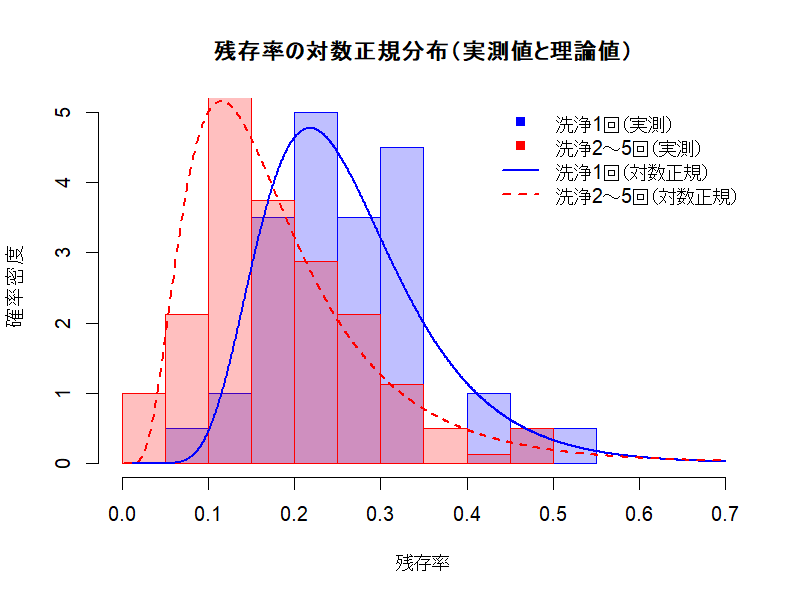
\includegraphics[width=0.85\linewidth]{fig/lognormal_distribution_with_data.png}
  \caption{残存率の対数正規分布（実測値と理論値）}
  \label{fig:lognorm_residual}
\end{figure}

以上より、洗浄条件ごとに推定した残存率分布を
第7章の感染リスク評価の入力分布として使用する。

%--------------------------------------------------
\section{まとめ}
本章では、第5章で算出した掌面積で正規化されたウイルス残存率を用い、
洗浄条件の違いによる残存率の変化について統計的な解析を行った。
はじめに、被験者および左右の手による影響を確認するため、洗浄回数ごとに
二元配置分散分析を実施した。その結果、被験者間差、左右差、およびそれらの
交互作用のいずれについても有意な差は認められなかった。このことから、
本研究で得られた標準化残存率は、個人差や左右差の影響を大きく受けるものではなく、
同一の集団として取り扱うことが可能であると判断した。

次に、洗浄回数がウイルス残存率に与える影響を評価するため、一元配置分散分析および 
Tukey 法による多重比較を行った。その結果、洗浄1回目と洗浄2回目以降の条件の間に有意な差が認められた
一方で、洗浄2回目から5回目の間では有意な差は認められなかった。この結果から、
初回の洗浄によってウイルスの大部分が除去され、2回目以降の洗浄による追加的な除去効果は限定的であることが示唆された。

以上の結果を踏まえ、本研究では洗浄条件を「洗浄1回目」と「洗浄2～5回目」の2群に分類して取り扱うことが妥当であると判断した。
さらに、これらの残存率データについて正規性を検定したところ正規分布には従わないことが確認されたため、
対数正規分布を仮定して確率密度分布関数の推定を行った。得られた分布は、実測値の分布傾向を良好に再現しており、
ウイルス残存率を確率的に取り扱う上で適切であると考えられる。

本章で得られた洗浄条件別のウイルス残存率分布は、
次章における感染リスク評価において重要な入力データとなる。
第7章では、これらの分布を用いてモンテカルロシミュレーションを実施し、
洗浄後に残存するウイルスによる感染リスクについて定量的な評価を行う。
